\chapter{Conjuntos}

\section{Noção de Conjunto}


Um conjunto é uma coleção qualquer de objetos formado por elementos. Um objeto \textbf{a} qualquer pode ser elemento de determinado conjunto $A$ ou não.


\begin{center}
	Quando \textbf{a} pertençe a $A$ escrevemos:
\end{center}
 	$$a \in A$$
 	
\begin{center}
	Quando \textbf{a} não pertençe a $A$ escrevemos:
\end{center}
	$$a \not\in A$$
	
	
\section{Conjuntos Númericos}

\subsection{Conjunto  dos Números Naturais $\mathbb{N}$}

O conjunto dos números naturais, simbolizado por $\mathbb{N}$ é o seguinte conjunto:

$$\mathbb{N} = \{0 \, ; \, 1\, ; \,2\, ; \,3\, ; \,4\,; \, ...\}$$

\textbf{Observações:}
\begin{itemize}
\item Quando $0 \not\in \mathbb{N}$ escrevemos $\mathbb{N}^*$.
$$\mathbb{N}^* = \{ 1\, ; \,2\, ; \,3\, ; \,4\, ; \, ...\}$$

\end{itemize}

\subsection{Conjunto  dos Números Inteiros $\mathbb{Z}$}

O conjunto dos números inteiros, simbolizado por $\mathbb{Z}$ é o seguinte conjunto:

$$\mathbb{Z} = \{...\,;\,-4\,;\,-3\,;\,-2\,;\,-1\,;\,0 \, ; \, 1\, ; \,2\, ; \,3\, ; \,4\, ; \, ...\}$$


\subsection{Conjunto  dos Números Racionais $\mathbb{Q}$}

O conjunto dos números racionais, simbolizado por $\mathbb{Q}$ é o conjunto das frações $\dfrac{a}{b}$ tal que $a \in \mathbb{Z}$ e $b \in \mathbb{Z}^*$.

$$\mathbb{Q} = \{...\,;\,-2\,;\,-1\,;\, -\frac{1}{2} \,;\,0 \, ; \, 1\, ;\,\frac{3}{2} \,; \,2\,; \, ...\}$$
\subsection{Conjunto  dos Números Irracionais $\mathbb{I}$}

O conjunto dos números irracionais, simbolizado por $\mathbb{I}$ é o conjunto dos números cuja representação com infinitas casas decimais não é periódica. Exemplo: $\sqrt{2};\,\sqrt{3};\,\pi$


\subsection{Conjunto  dos Números Reais $\mathbb{R}$}

O conjunto dos números reais, simbolizado por $\mathbb{R}$ é o conjunto formado por todos os números com representação decimal, decimais exatas e periódicas e as decimais não exatas e não periódicas.
\begin{figure}[H]
	\centering
	
	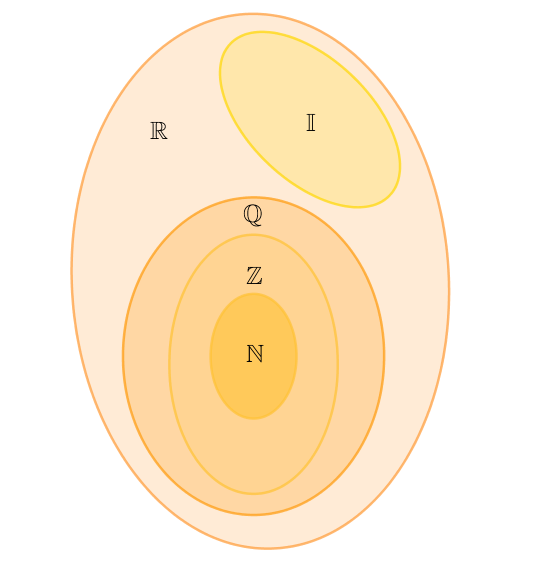
\includegraphics[scale=3.5]{imagens/conjunto-reais.png}

\end{figure}


\section{Intervalos Reais}

Dados dois números reais, $a$ e $b$, com $a < b$, temos:
\begin{itemize}
\begin{center}
	 Intervalo aberto
\end{center}

$$]a,b[ = \{x \in \mathbb{R}|\, a < x < b \}$$
\begin{figure}[H]
	\centering
	
	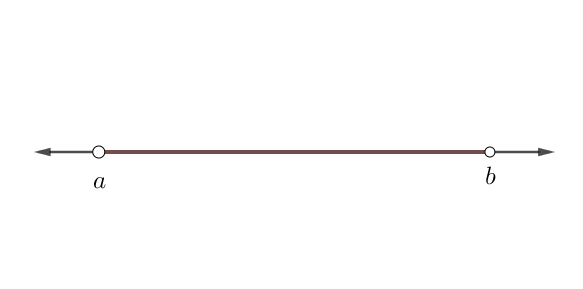
\includegraphics[scale=3.5]{imagens/intervalo-aberto.png}

\end{figure}

\begin{center}
	Intervalo fechado
\end{center}

$$[a,b] = \{x \in \mathbb{R}|\, a \leq x \leq b \}$$
\begin{figure}[H]
	\centering
	
	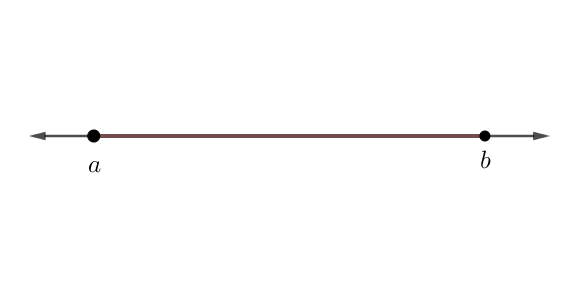
\includegraphics[scale=3.5]{imagens/intervalo-fechado.png}

\end{figure}
\begin{center}
	Intervalo fechado à esquerda e aberto à direita
\end{center}

$$[a,b[ = \{x \in \mathbb{R}|\, a \leq x < b \}$$
\begin{figure}[H]
	\centering
	
	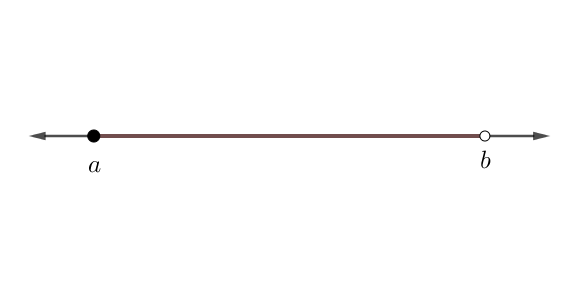
\includegraphics[scale=3.5]{imagens/intervalo-fechado-esquerda.png}

\end{figure}

\begin{center}
	Intervalo fechado à direita e aberto à esquerda
\end{center}

$$]a,b] = \{x \in \mathbb{R}|\, a < x \leq b \}$$
\begin{figure}[H]
	\centering
	
	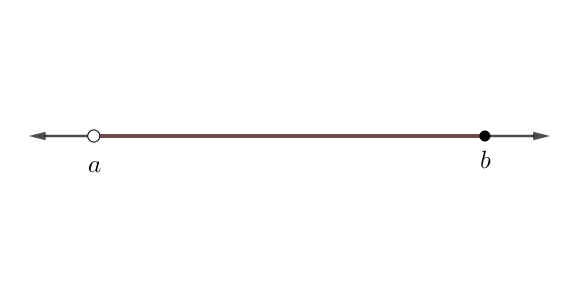
\includegraphics[scale=3.5]{imagens/intervalo-fechado-direita.png}

\end{figure}

\begin{center}
	Semirreta esquerda, fechada, de origem $b$
\end{center}

$$]-\infty,b] = \{x \in \mathbb{R}|\,  x \leq b \}$$
\begin{figure}[H]
	\centering
	
	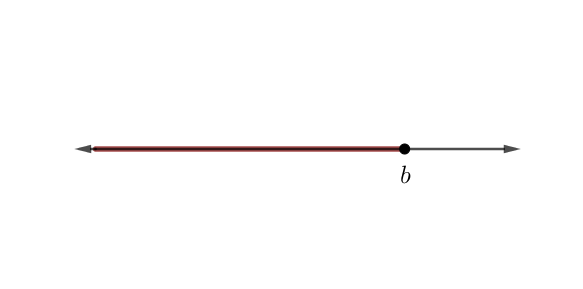
\includegraphics[scale=3.5]{imagens/semi-b-esquerda-fechada.png}

\end{figure}

\begin{center}
	Semirreta esquerda, aberta, de origem $b$
\end{center}

$$]-\infty,b[ = \{x \in \mathbb{R}|\,  x < b \}$$
\begin{figure}[H]
	\centering
	
	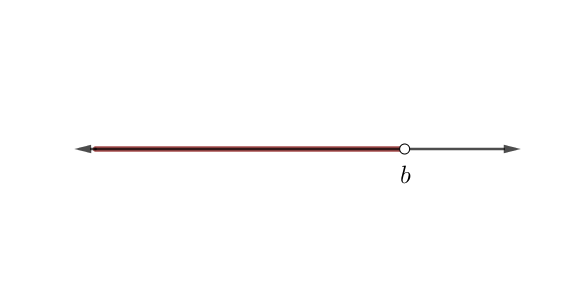
\includegraphics[scale=3.5]{imagens/semi-b-esquerda-aberta.png}

\end{figure}
\begin{center}
	Semirreta direita, fechada, de origem $a$
\end{center}

$$[a,+\infty[ = \{x \in \mathbb{R}|\,  x \geq a \}$$
\begin{figure}[H]
	\centering
	
	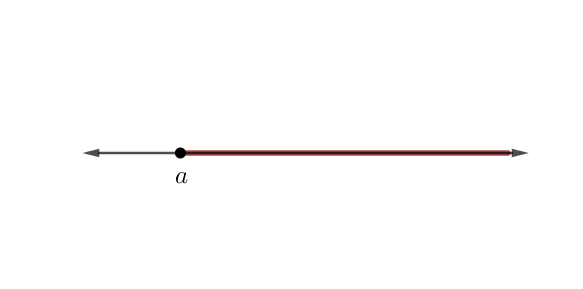
\includegraphics[scale=3.5]{imagens/semi-a-direita-fechada.png}

\end{figure}
\begin{center}
	Semirreta direita, aberta, de origem $a$
\end{center}

$$]a,+\infty[ = \{x \in \mathbb{R}|\,  x > a \}$$
\begin{figure}[H]
	\centering
	
	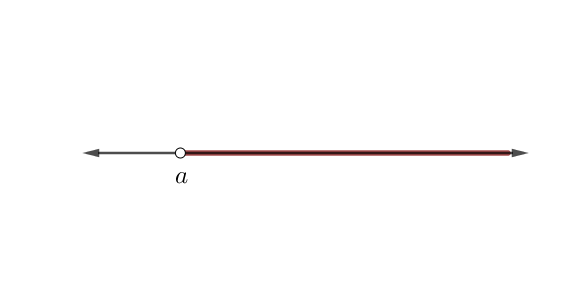
\includegraphics[scale=3.5]{imagens/semi-a-direita-aberta.png}

\end{figure}
\begin{center}
	Reta real
\end{center}

$$]-\infty,+\infty[ = \mathbb{R}$$
\begin{figure}[H]
	\centering
	
	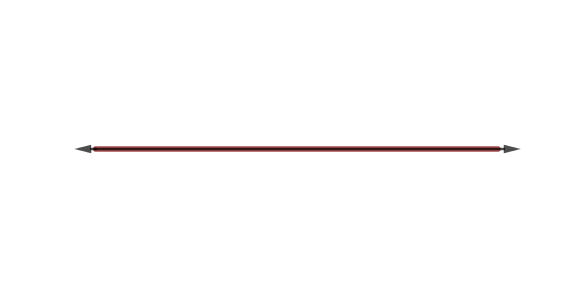
\includegraphics[scale=3.5]{imagens/reta-real.png}

\end{figure}

\end{itemize}

